\documentclass[xcolor=table]{beamer}

\usepackage[serbianc]{babel}
\usepackage{graphicx}
\usepackage{makeidx}
\usepackage{listings}
\usepackage{adjustbox}
%\usepackage[table,xcdraw]{xcolor}

\hypersetup{unicode}
\makeindex
\usefonttheme{professionalfonts}
\usetheme{CambridgeUS}

\title{Spectre \& Meltdown}
\author{Борисав Живановић}

\begin{document}

    \begin{frame}
        \maketitle
    \end{frame}

    \begin{frame}{Садржај}
        \begin{enumerate}
            \item Архитектура и микроархитектура
            \item Кеширање
            \item Предвиђање гранања и прекоредно извршавање
            \item Основни мехнанизми изолације
            \item Употреба кеша као side-channel
            \item Spectre
            \item Meltdown
        \end{enumerate}
    \end{frame}
    
    \section{Архитектура и микроархитектура}
    
    \begin{frame}{Шта рачунар заиста зна да ради?}
        \begin{itemize}
            \item Језик рачунара: \textbf{скуп инструкција} (енгл. ISA, Instruction Set Architecture)
            \item Аритметичке операције: \textbf{add}, \textbf{sub}, \textbf{div}, \textbf{mul}, …
            \item Померање података:
            \begin{itemize}
                \item са улазног уређаја у меморију
                \item из меморије на излазни уређај
                \item са једне меморијске локације на другу
            \end{itemize}
            \item Условно гранање: извршавање кода уколико је логички услов испуњен
        \end{itemize}
    \end{frame}
    
    \begin{frame}{Условно гранање}
        \begin{itemize}
            \item Кључни механизам - омогућава имплементацију \textbf{било ког} алгоритма
            \item Концпети виших програмских језика као што су \textbf{if}, \textbf{else}, \textbf{for}, \textbf{while}, \textbf{switch} се своде на условно гранање
        \end{itemize}
    \end{frame}
    
    \begin{frame}{Instruction Set Architecture}
        \begin{itemize}
            \item Представља слој апстракције изнад микроархитектуре
            \item Главна разлика између различитих ISA је у количини логике коју појединачна инструкција може да садржи
            \item Подела: CISC (Complex Instruction Set Computer), RISC (Reduced Instruction Set Computer)
            \item x86 је иницијално био класична CISC архитектура
            \item Данас x86 инструкције на нивоу ISA се преводе у \textbf{микроинструкције} налик на RISC инструкције
            \begin{itemize}
                \item ово се дешава на нивоу микроархитектуре и програмер тога није свестан!
            \end{itemize}
        \end{itemize}
    \end{frame}
    
    \begin{frame}{Микроархитектура}
        \begin{itemize}
            \item Представља конкретну имплементацију ISA
            \item Замисао је да се кроз време имплементација побољшава, а да се задржи компатибилност са постојећим софтвером
            \item Неке разлике између различитих микроархитектура:
            \begin{itemize}
                \item параметри кеша (капацитет, асоцијативност, величина линије, број нивоа)
                \item број језгара
                \item подршка за механизме који крше секвенцијалан модел извршавања
            \end{itemize}
        \end{itemize}
    \end{frame}
    
    \section{Кеширање}
    
    \begin{frame}[allowframebreaks]{Меморијска хијерархија}
        \textit{
            Ideally one would desire an indefinitely large
            memory capacity such that any particular... word
            would be immediately available... We are... forced
            to recognize the possibility of constructing a
            hierarchy of memories each of which has greater
            capacity than the preceding but which is less
            quickly accessible.
        }

        \begin{flushright}
            \textbf{Burks, Goldstine, von Neumann} (1946)
        \end{flushright} 

        \framebreak
        
        \begin{itemize}
            \item Проблем: не постоји бесконачно брза и бесконачно велика меморија
            \item Чињеница: постоје технологије меморије које омогућавају релативно велики капацитет, по цену релативно мале брзине
            \begin{itemize}
                \item ...као и обрнуто!
                \item брзина и капацитет меморије су, по правилу, обрнуто сразмерни
            \end{itemize}
            \item Да ли је могуће добити највећи капацитет уз највећу брзину, по најмањој цени?
            \item Меморијска хијерархија нам ово \textit{донекле} омогућава
            \begin{itemize}
                \item цена: \textit{приближно} најспорија меморија
                \item брзина: \textit{приближно} најбржа меморија
            \end{itemize}
        \end{itemize}
        
        \framebreak

        \begin{figure}
            \centering
            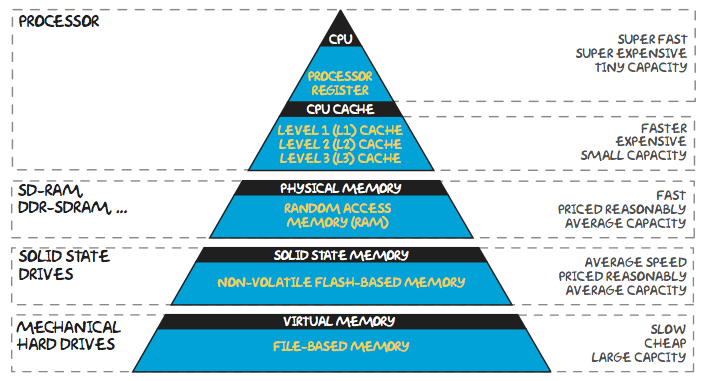
\includegraphics[width=\textwidth,height=0.7\textheight,keepaspectratio]{images/mem1.jpg}
            \label{fig:mem1}
        \end{figure}
    \end{frame}
    
    \begin{frame}[allowframebreaks]{Локалитет}
        \begin{itemize}
            \item \textbf{Просторни локалитет}: уколико је некој локацији приступљено, вероватно ће бити приступљено и суседним локацијама
            \begin{itemize}
                \item пример: приступање суседним елементима низа, извшавање наредних инструкција
            \end{itemize}
            \item \textbf{Временски локалитет}: уколико је некој локацији приступљено, вероватно ће јој бити приступљено у скоријем временском периоду
            \begin{itemize}
                \item пример: позив методе у петљи, приступ елементима \textit{linked list}
            \end{itemize}
            \item Мерењима је доказано да програми поштују наведене особине
        \end{itemize}
        
        \framebreak

        \begin{itemize} 
            \item Цео меморијски подсистем је оптимизован за програме који поштују локалитет
            \begin{itemize}
                \item уколико покренемо заједно један програм који поштује локалитет (Matlab) са другим који не поштује (GCC), може да дође до давања предности оном који поштује! 
            \end{itemize}
            \item Поједине специјализоване архитектуре избацују кеш меморију уколико није могуће направити решење које поштује локалитет
            \begin{itemize}
                \item у овом случају, кеширање би успорило програм
            \end{itemize}
            \item Занимљивост: постоје случајеви у којима су операције над \textit{array list} брже него над \textit{linked list}, јер иако је временска сложеност операција већа, операције се далеко брже извршавају уколико је цео низ у кешу!
        \end{itemize}
    \end{frame}
    
    \begin{frame}[allowframebreaks]{Кеш меморија}
        \begin{itemize}
            \item Налази се у процесору, најчешће имплементирана у SRAM технологији
            \item Чува тренутно потребан подскуп радне меморије програма
            \begin{itemize}
                \item подскуп се динамички одређује уз претпоставку локалитета
            \end{itemize}
            \item Програмер не мора да буде свестан конкретне имплементације кеша
            \begin{itemize}
                \item али је то, у одређеним случајевима, пожељно
                \item постоје инструкције које омогућавају измену стања кеша (CLFLUSH, PREFETCHW)
            \end{itemize}
            \item Сваки меморијски приступ мора да прође кроз кеш
        \end{itemize}
        
        \framebreak

        \begin{figure}
            \centering
            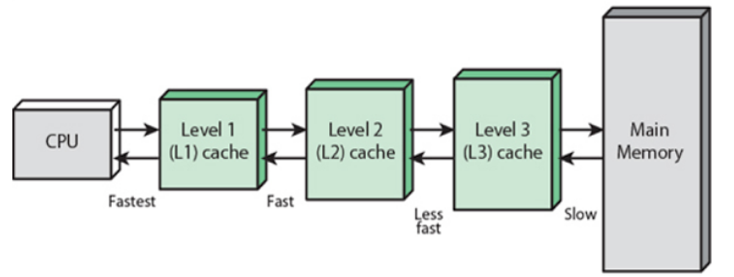
\includegraphics[width=\textwidth,height=\textheight,keepaspectratio]{images/mem2.jpg}
            \label{fig:mem2}
        \end{figure}
        
        \framebreak
        
        \begin{itemize}
            \item \textbf{Cache hit}: тражени податак је пронађен у кешу
            \item \textbf{Cache miss}: тражени податак није пронађен у кешу
            \item \textbf{Hit time}: време које је потребно да се утврди да ли је тражени податак у кешу
            \item \textbf{Miss time}: време које је потребно да се тражени податак добави у кеш
        \end{itemize}
    \end{frame}
    
    \section{Предвиђање гранања и прекоредно извршавање}
    \subsection{Предвиђање гранања}
    
    \begin{frame}{Предвиђање гранања}
        \begin{itemize}
            \item \textbf{if(x < y) \{...\} else \{...\}}
            \item Променљиве \textbf{x} и \textbf{y} представљају вредности из радне меморије 
            \item Одређивање гране коју треба извршити није могуће док обе вредности не буду добављене у кеш
            \item Условно гранање често изазива \textbf{cache miss}
            \begin{itemize}
                \item ...и на тај начин зауставља рад процесора
            \end{itemize}
            \item Идеја:
            \begin{itemize}
                \item извршавање гране за коју се претпоставља да ће бити изабрана док се чека IO
                \item чување или одбацивање резултата након утврђивања да ли је извршавање гране требало да се деси
            \end{itemize}
        \end{itemize}
    \end{frame}
    
    \subsection{Прекоредно извршавање}
    
    \begin{frame}[fragile]{Прекоредно извршавање}
        \begin{itemize}
            \item{
                \begin{lstlisting}[language=java]
a1 = b1 + c1;
a2 = b2 + c2;
a = a1 + a2;
                \end{lstlisting}
            }
            
            \item Шта ако су вредности \textbf{b2} и \textbf{c2} у кешу, а потребно је прво сачекати добављање \textbf{b1} и \textbf{c1}?
            \item У секвенцијалном моделу извршавања, процесор би био заустављен
            \item Идеја:
            \begin{itemize}
                \item на нивоу ISA задржавамо секвенцијални модел извршавања
                \item на нивоу микроархитектуре инструкције извршавамо у редоследу који зависи од доступних података
                \item резултат програма мора остати исти!
            \end{itemize}
        \end{itemize}
    \end{frame}
    
    \section{Основни механизми изолације}
    
    \begin{frame}{Индирекција}
        \begin{itemize}
            \item Било који проблем у рачунарству може бити решен још једним нивоом индирекције, осим наравно проблема превише индирекција (David J. Wheeler)
            \item Индирекција омогућава имплементацију контроле приступа
            \item Извршавање \textbf{акције} мора да одобри \textbf{посредник} који дефинише правила приступа
        \end{itemize}
    \end{frame}
    
    \begin{frame}[allowframebreaks]{Контрола приступа у хардверу}
        \begin{itemize}
            \item Рачунар без контроле приступа би донекле био употребљив у једнокорисничком окружењу
            \begin{itemize}
                \item ...али неупотребљив у вишекорисничком
                \item чак и у једнокорисничком окружењу, одсуство изолације процеса представља велику опасност
            \end{itemize}
            \item Основне градивне блокове је неопходно имплементирати у хардверу
            \begin{itemize}
                \item софтвер можда неће бити рад да сарађује!
            \end{itemize}
            \item Кључни механизми: режими рада процесора, виртуелна меморија
            \item Додатне контроле се имплементирају у кернелу
            \begin{itemize}
                \item пријављивање корисника на систем, пермисије за приступ фајловима
            \end{itemize}
        \end{itemize}
        
        \framebreak
        
        \begin{figure}
            \centering
            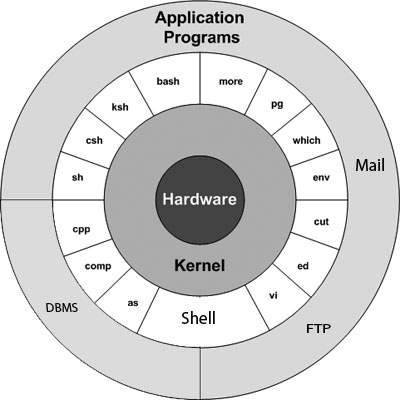
\includegraphics[width=\textwidth,height=0.8\textheight,keepaspectratio]{images/unix_architecture.jpg}
            \label{fig:unix_architecture.jpg}
        \end{figure}
    \end{frame}
    
    \begin{frame}{Режими рада процесора}
        \begin{itemize}
            \item Привилеговани: IO, меморијске табеле, табеле прекида
            \begin{itemize}
                \item кернел
            \end{itemize}
            \item Неривилеговани: аритметичко/логичке операције, условно гранање, ограничен приступ меморији, системски позив
            \begin{itemize}
                \item кориснички софтвер
            \end{itemize}
            \item Прелазак из непривилегованог у привилеговани режим је могућ приликом прекида или системског позива
            \item Кернел одбија захтев уколико кориснички процес нема потребне привилегије и убија га
        \end{itemize}
    \end{frame}
    
    \begin{frame}[allowframebreaks]{Виртуелна меморија}
        \begin{itemize}
            \item
        \end{itemize}
        
        \framebreak
        
        \begin{figure}
            \centering
            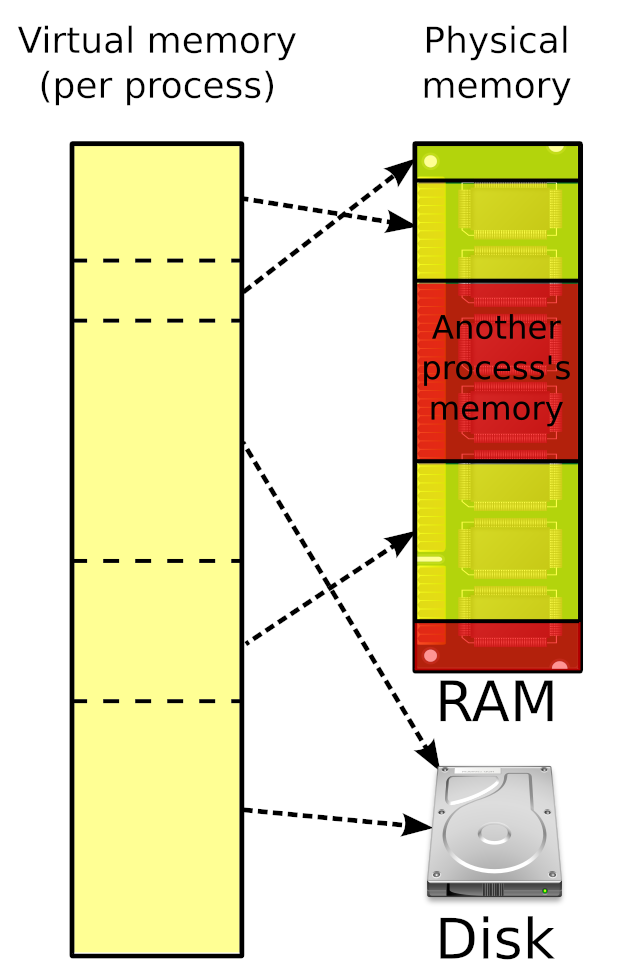
\includegraphics[width=\textwidth,height=0.8\textheight,keepaspectratio]{images/virtmem.png}
            \label{fig:virtmem}
        \end{figure}
    \end{frame}
    
    \begin{frame}{Покретање оперативног система}
        \begin{itemize}
            \item Процесор се буди у привилегованом режиму
            \item Учитава се кернел
            \item Иницијализују се табеле прекида
            \item Иницијализују се меморијске табеле
            \item Контрола се предаје корисничким програмима, прелази се у непривилегован режим
            \item Овако подешен посредник више није могуће уклонити или заобићи
            \begin{itemize}
                \item ...под претпоставком да нема багова у имплементацији кернела и хардвера
            \end{itemize}
        \end{itemize}
    \end{frame}
    
    \begin{frame}[allowframebreaks]{Употреба кеша као side-channel}
        \begin{itemize}
            \item До сада смо причали о механизмима који нам омогућавају безбедно дељење рачунара и побољшање перформанси секвенцијалног модела
            \item Безбедност и перформасе су често супротни захтеви у дизајну!
            \item Заједничко за оба напада је да извршавају недозвољен меморијски приступ \textbf{спекулативно}
            \begin{itemize}
                \item пошто је извршавање \textbf{спекулативно}, процесор ефекте чува/одбацује накнадно
                \item комплетно одбацивање резултата није могуће
                \item стање ISA се успешно поништава, али остаје видљиво стање микроархитектуре (вредности у кешу!)
            \end{itemize}
            \item Добијену вредност кодирају као довлачење линије у кеш
            \item Добијену вредност декодирају као проверу присуства линије у кешу
        \end{itemize}
        
        \framebreak
        
        \begin{itemize}
            \item Директан недозвољен приступ није могућ
            \item Проблем настаје код спекулативног извршавања, јер процесор не зна да ли да баци грешку
            \item Приступ вредности учитане у кеш је видно брже од вредности из радне меморије
            \item Алгоритам:
            \begin{itemize}
                \item алоцирамо низ
                \item изазивамо недозвољен приступ меморији
                \item приступамо елементу низа чији индекс одговара тајној вредности
                \item итерирамо кроз низ и меримо време потребно за приступ индексима
                \item уклањамо цео низ из кеша и приступамо наредној недозвољеној адреси
            \end{itemize}
        \end{itemize}
        
        \framebreak
        
        \begin{table}[]
            \begin{tabular}{|l|l|l|}
                \hline
                елемент                             & кодирана вредност        & време приступа                \\ \hline
                \rowcolor[HTML]{FD6864} 
                a{[}x * 0{]}                        & 0                        & 300 ns                        \\ \hline
                \rowcolor[HTML]{FD6864}
                a{[}x * 1{]}                        & 1                        & 300 ns                        \\ \hline
                \rowcolor[HTML]{67FD9A} 
                a{[}x * 2{]}                        & 2                        & 5 ns                          \\ \hline
                \rowcolor[HTML]{FD6864}
                a{[}x * 3{]}                        & 3                        & 300 ns                        \\ \hline
                ...                                 & ...                      & ...                           \\ \hline
                \rowcolor[HTML]{FD6864}
                a{[}x * 254{]}                      & 254                      & 300 ns                        \\ \hline
            \end{tabular}
        \end{table}
        
        Скалирање за вредност \textbf{x} је неопхондно јер би у супротном једна линија кеша представљала 16 вредности, јер је \textbf{int} ширине 32 бита,
        а величина линије кеша је углавном 64 бајта 
    \end{frame}
    
    \begin{frame}{Литература}
        \begin{itemize}
            \item Spectre Attacks: Exploiting Speculative Execution
            \item Meltdown: Reading Kernel Memory from User Space
            \item Computer Organization and Design: The Hardware/Software Interface, David A. Patterson \& John L. Hennessy
            \item Системски софтвер (презентације), Иван Нејгебауер
            \item Operating Systems: Internals and Design Principles, William Stallings
        \end{itemize}
    \end{frame}

\end{document}
